\section{ПРОГРАММЫ И БИБЛИОТЕКИ ДЛЯ РЕШЕНИЯ ОДУ}

Программ для решения ОДУ достаточно много. На рисунке \ref{fig:programs} приведены
некоторые популярные программы и библиотеки для решения дифференциальных
уравнений. Рассмотрим детально достоинства и недостатки каждой из них.

\begin{figure}
    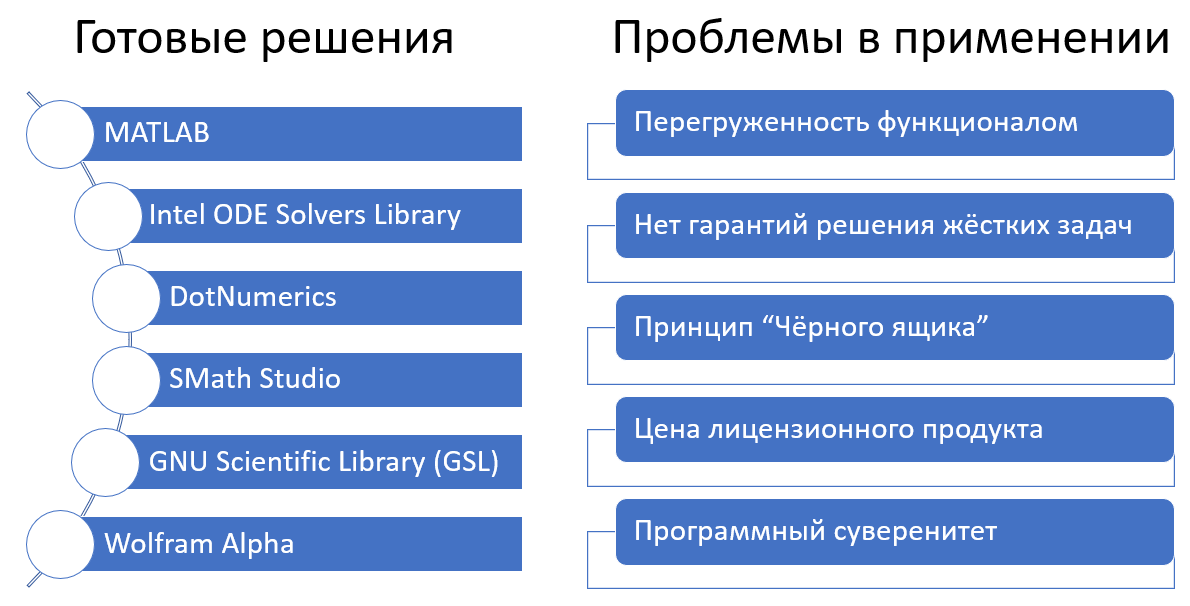
\includegraphics[width=15cm]{2-01-programs}
    \caption{Программы и библиотеки}
    \label{fig:programs}
\end{figure}

Наиболее распространённый программный продукт ~--- пакет программ для решения задач технических вычислений MATLAB. Первый выпуск состоялся в 1984 году. Пакет используют
более миллиона инженерных и научных работников, он работает на большинстве современных операционных систем, включая Linux, macOS и
Windows. Разработчиком является американская компания The MathWorks. Написан с использованием языков программирования С, С++, Fortran,
Java.

Для решения ОДУ MATLAB предлагает следующие функции:
\begin{itemize}
    \item ode23() ~--- метод решения нежёстких дифференциальных уравнений; метод низкого порядка,
    \item ode45() ~--- метод решения нежёстких дифференциальных уравнений; метод среднего порядка,
    \item ode113() ~--- метод решения нежёстких дифференциальных уравнений; метод переменного порядка,
    \item ode15s() ~--- метод решения жёстких дифференциальных уравнений; метод переменного порядка,
    \item ode23s() ~--- метод решения жёстких дифференциальных уравнений; метод низкого порядка.
\end{itemize}

MATLAB имеет свой собственный язык программирования для подготовки данных и большую библиотеку для работы с матрицами, построения
графиков и численных вычислений. Однако он является довольно тяжёлым, имеет низкую скорость работы и не
подходит для решения задач химической кинетики. Помимо этого, в бесплатной версии недостаточно инструментов, а цена полной версии
несолько завышена.

Альтернативу пакету MATLAB может составить отечественная программа SMath Studio, разработанная ООО "ЭсМат".
SMath Studio предназначена для вычисления математических выражений и построения графиков функций. Бета-версия была выпущена в 2018
году и работа над обновлениями продолжается в настоящее время. Работа с интерфейсом
программы напоминает работу с обычным листом бумаги, так как все математические выражения в ней записываются не в строчку текстом,
а в графическом, удобном для человека, виде (по аналогии с системой Mathcad).

Для решения ОДУ в SMath Studio реализованы следующие методы:

\begin{itemize}
    \item неявный метод Эйлера (2-го порядка),
    \item явный метод Рунге-Кутты (классический 4-го порядка).
\end{itemize}

Ограниченное количество методов для решения ОДУ не позволяет использовать её для решения жёстких задач и задач химичесой кинетики
в частности.

В дополнение предыдущей программы можно посмотреть библиотеку Intel ODE Solver Library.
Библиотека написана на языке C со всеми вытекающими отсюда зависимостями. Доступны 32- и 64-разрядные версии.

В этой библиотеке следует выделить следующие программы и функции:
\begin{itemize}
    \item rkm9st() ~--- функция для решения нежёстких и средне-жёстких систем ОДУ с использованием явного метода, который основан на
        методе Мерсона 4-го порядка и многоступенчатом методе 1-го порядка, включающем до 9 этапов с контролем устойчивости,
    \item mk52lfn() ~--- специализированная процедура для решения жёстких систем ОДУ с использованием неявного метода, основанного
        на L-стабильном (5,2)-методе с числовой матрицей Якоби, которая вычисляется с помощью процедуры,
    \item mk52lfa() ~--- специализированная программа для решения жёстких систем ОДУ с использованием неявного метода, основанного на
        L-stable (5,2)-методе с численным или аналитическим вычислением матрицы Якоби. Пользователь должен предоставить процедуру для
        этого вычисления,
    \item rkm9mkn() ~--- специализированная процедура для решения систем ОДУ с переменной или априори неизвестной жёсткостью;
        автоматически выбирает явную или неявную схему на каждом шаге и при необходимости вычисляет числовую матрицу Якоби,
    \item rkm9mka() ~--- специализированная подпрограмма для решения систем ОДУ с переменной или априори неизвестной жёсткостью;
        автоматически выбирает явную или неявную схему на каждом шаге. Пользователь должен предоставить процедуру для численного или
        аналитического вычисления матрицы Якоби.
\end{itemize}

У данной библиотеки есть хороший набор для решения нежёстких задач, есть автоматический выбор явного или неявного шага на каждой
итерации, однако для решения жёстких задач требуется дополнительно вводить Якобиан, что достаточно проблематично.

GNU Scientific Library (или GSL) ~--- это библиотека, написанная на языке программирования C для численных вычислений в прикладной
математике и науке. GSL является частью проекта GNU (Массачусетский технологический институт, США) и распространяется на условиях
лицензии GPL.
Первый релиз состоялся в 1996 году.

GSL используется, в частности, в таком программном обеспечении, как PSPP и Perl Data Language.

Следует отметить следующие достаточно хорошо известные явные методы:
\begin{itemize}
    \item rk2() ~--- явный метод Рунге-Кутты (2, 3),
    \item rk4() ~--- явный 4-й порядок (классический) Рунге-Кутты. Оценка погрешности осуществляется методом удвоения шага,
    \item rkf45() ~--- явный метод Рунге-Кутты-Фельберга (4, 5),
    \item rkck() ~--- явный метод Рунге-Кутты Кэш-Карпа (4, 5),
    \item rk8pd() ~--- явный метод Рунге-Кутты Принца-Дорманда (8, 9).
\end{itemize}

Среди неявных методов можно отметить методы, требующие построение Якобиана до 4-го порядка и большой набор многошаговых методов типа
Адамса:
\begin{itemize}
    \item rk1imp() ~--- неявный гауссовский метод Рунге-Кутты первого порядка. Также известен как неявный метод Эйлера или обратный
        метод Эйлера. Оценка погрешности осуществляется методом удвоения шага. Для этого алгоритма требуется якобиан,
    \item rk2imp() ~--- неявный гауссовский метод Рунге-Кутты второго порядка. Также известно как неявное правило средней точки. Оценка
        погрешности осуществляется методом удвоения шага. Для этого шагового двигателя требуется якобиан,
    \item rk4imp() ~--- неявный гауссов Рунге-Кутта 4-го порядка. Оценка погрешности осуществляется методом удвоения шага. Для этого
        алгоритма требуется якобиан,
    \item bsimp() ~--- неявный метод Булирша-Стоера (многошаговый). Этот метод, как правило, подходит для сложных задач. Для этого
        шагового двигателя требуется якобиан,
    \item msadams() ~--- линейный многоступенчатый метод Адамса с переменным коэффициентом в форме Nordsieck. Этот шаговый процессор
        использует явные методы Адамса-Башфорта (предсказатель) и неявные методы Адамса-Моултона (корректор) в режиме функциональной
        итерации $P(EC)^m$. Порядок методов динамически варьируется от 1 до 12,
    \item msbdf() ~--- метод линейной многоступенчатой формулы обратного дифференцирования с переменным коэффициентом (BDF) в форме
        Nordsieck. Этот шаговый преобразователь использует явную формулу BDF в качестве предиктора и неявную формулу BDF в качестве
        корректора. Для решения системы нелинейных уравнений используется модифицированный итерационный метод Ньютона. Порядок методов
        динамически варьируется от 1 до 5. Этот метод, как правило, подходит для сложных задач. Для этого шагового двигателя требуется
        якобиан.
\end{itemize}

В данной библиотеке большое количество как явных, так и неявных методов, но для невных методов как и в библиотеке Intel ODE Solver
Library требуется самостоятельное вычисление Якобиана. Недостаток именно библиотечного вида заключается в том, что надо писать модули
обращения и модули обработки результата.

Следующей библиотекой для рассмотрения является DotNumerics. Она включает в себя числовую библиотеку для .NET. Библиотека написана на
чистом C\# и содержит более 100 000 строк кода с
самыми передовыми алгоритмами для линейной алгебры, дифференциальных уравнений и задач оптимизации. Библиотека линейной алгебры
включает CSLapack, Cabelas и CSEispack, эти библиотеки являются переводом с Fortran на C\# LAPACK, BLAS и EISPACK соответственно.

Основные решатели для нежёстких систем:
\begin{itemize}
    \item ExplicitRK45() ~--- решает задачу с начальными значениями для нелинейных обыкновенных дифференциальных уравнений, используя
        явный метод Рунге-Кутты порядка (4)5,
    \item AdamsMoulton() ~--- решает начальную задачу для нелинейных обыкновенных дифференциальных уравнений с использованием метода
        Адамса-Моултона.
\end{itemize}

Решатели для жёстких систем:
\begin{itemize}
    \item ImplicitRK5() ~--- решает начальную задачу для жёстких обыкновенных дифференциальных уравнений с использованием неявного
        метода Рунге-Кутты порядка 5,
    \item GearsBDF() ~--- решает начальную задачу для жёстких обыкновенных дифференциальных уравнений с использованием многошагового
        метода BDF Gear.
\end{itemize}

В данной библиотеке представлено небольшое число методов решения ОДУ до 5 порядка точности. В основном эта библиотека обслуживает
не только задач дифференциальных уравнений, но и задачи линейной алгебры, в том числе задачи оптимизации, поэтому она содержит мало методов
для решения моей задачи.

Отметим так же систему Wolfram Alpha. Это база знаний и набор вычислительных алгоритмов, вопросно-ответная
система.

Wolfram Alpha способен переводить данные между различными единицами
измерения, системами счисления, подбирать общую формулу последовательности, находить возможные замкнутые формы для приближенных
дробных чисел, вычислять суммы, пределы, интегралы, решать уравнения и системы уравнений, производить операции с матрицами, определять
свойства чисел и геометрических фигур. Отдельного внимания стоит парсинг математических выражений.

В частности система Wolfram Alpha способна решать ОДУ стандартными явными методами:
\begin{itemize}
    \item метод Эйлера (2-го порядка),
    \item метод средних точек, модифицированный метод Эйлера,
    \item метод Хойна, вариант модифицированного метода Эйлера,
    \item метод Рунге-Кутты 3-го порядка,
    \item метод Рунге-Кутты (классический 4-го порядка),
    \item метод Рунге-Кутты-Фалберга,
    \item метод Дормана-Принца.
\end{itemize}

Система Wolfram Alpha является облачной. Это означает, что для работы с ней необходимо постоянное подключение к интернету. Ещё
одним недостатком является наличие платного функционала и отсутствие готовых модулей для создания и решения СДУ химической кинетики.

Несмотря на большое число программ и библиотек для решение ДУ, появилась потребность в создании программы (с большим выбором расчетных
схем) для решения (в то числе и) жёстких систем ДУ для задач химической кинетики.